\begin{pastexam}[label={px:gk3-111-ds-04}]{高考三級資訊處理 111 年 第四題}
（申論；25 分）

用 G = (V, E)表示一個無方向性圖形，其中 V 是點的集合，E 是一組節點（Vertices）形成邊及對應權重
（Weights）所組成的集合。今有一圖形 G = (V, E)，V = \{0, 1, 2, 3, 4, 5\}，圖形的邊與權重值以如下的
定義儲存對應連接矩陣(Adjacency matrix)表示中的值

\hspace*{1em}\#define\quad MAX\_EDGES\quad 100\\
\hspace*{1.5em}typedef\quad struct \{\\
\hspace*{8em}int\quad col;\\
\hspace*{8em}int\quad row;\\
\hspace*{8em}int\quad weight;\\
\hspace*{8em}\} edge;\\
\hspace*{1em}edge\quad a[MAX\_EDGES];

已知陣列 a 儲存對應連接矩陣相連接邊的內容如下：a = \{(3, 0, 2), (4, 0, 1), (5, 0, 20), (2, 1, 7),
(5, 1, 24), (3, 2, 15), (4, 2, 10), (5, 2, 25), (4, 3, 3)\}。請畫出陣列 a 所儲存的圖形，然後，利用
Prim 演算法從節點 0 開始依加入其它節點的順序，畫出此圖之最小擴張樹（Minimum spanning tree），並
計算其最低權重或成本值。（25 分）
\end{pastexam}

\begin{pastsoln}
\textbf{讀出邊。} 每一筆是 (col, row, weight)，表示鄰接矩陣第 row 列、第 col 行的元素，也就是
頂點 row 和頂點 col 之間有一條權重 weight 的邊。 圖是無向的，矩陣對稱，所以只存了一半
（每筆都是 row $<$ col）。 九筆對應九條邊：
\begin{center}
\begin{tabular}{ccccccccc}
\toprule
(0,3) & (0,4) & (0,5) & (1,2) & (1,5) & (2,3) & (2,4) & (2,5) & (3,4) \\
2 & 1 & 20 & 7 & 24 & 15 & 10 & 25 & 3 \\
\bottomrule
\end{tabular}
\end{center}

\textbf{圖形。}
\begin{center}
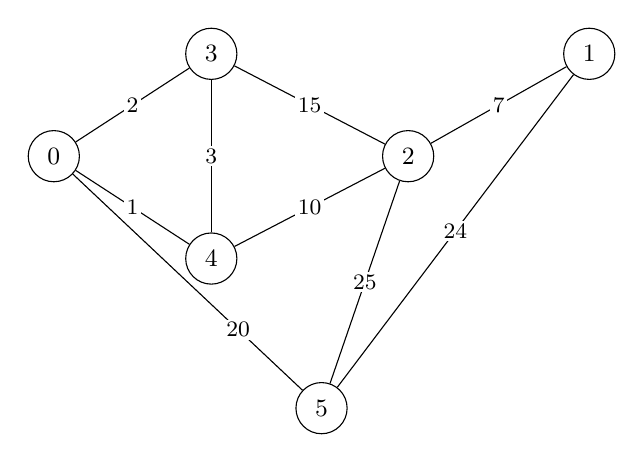
\begin{tikzpicture}[
    v/.style={circle, draw, minimum size=6.5mm, inner sep=0pt, font=\small},
    w/.style={fill=white, inner sep=1pt, font=\footnotesize}]
\node[v] (0) at (0,0) {0};
\node[v] (3) at (2,1.3) {3};
\node[v] (4) at (2,-1.3) {4};
\node[v] (2) at (4.5,0) {2};
\node[v] (1) at (6.8,1.3) {1};
\node[v] (5) at (3.4,-3.2) {5};
\draw (0) -- node[w] {2} (3);
\draw (0) -- node[w] {1} (4);
\draw (0) -- node[w, pos=0.72] {20} (5);
\draw (1) -- node[w] {7} (2);
\draw (1) -- node[w] {24} (5);
\draw (2) -- node[w] {15} (3);
\draw (2) -- node[w] {10} (4);
\draw (2) -- node[w] {25} (5);
\draw (3) -- node[w] {3} (4);
\end{tikzpicture}
\end{center}

\textbf{Prim，從節點 0 開始。} 每一步在「一端已在樹裡、一端不在」的邊裡挑最輕的，把另一端加進樹
（資結書第~24.3~節）。 下表列出每一步樹外各頂點目前最輕的連接邊（括號是樹裡那一端）：
\begin{center}
\begin{tabular}{clcl}
\toprule
步 & 樹外頂點的最輕連接邊 & 選的邊 & 樹裡的頂點 \\
\midrule
開始 & & & \{0\} \\
1 & 3:2(0), 4:1(0), 5:20(0) & (0,4) 1 & \{0, 4\} \\
2 & 2:10(4), 3:2(0), 5:20(0) & (0,3) 2 & \{0, 4, 3\} \\
3 & 2:10(4), 5:20(0) & (4,2) 10 & \{0, 4, 3, 2\} \\
4 & 1:7(2), 5:20(0) & (2,1) 7 & \{0, 4, 3, 2, 1\} \\
5 & 5:20(0) & (0,5) 20 & \{0, 4, 3, 2, 1, 5\} \\
\bottomrule
\end{tabular}
\end{center}
第 2 步之後 (3,4) 3 兩端都在樹裡，不能選；第 3 步時 2 可以經 (4,2) 10 或 (3,2) 15 連進來，選 10。
第 5 步 5 的三條邊是 20、24、25，選 (0,5) 20。

加入節點的順序：0, 4, 3, 2, 1, 5。 最小擴張樹：
\begin{center}
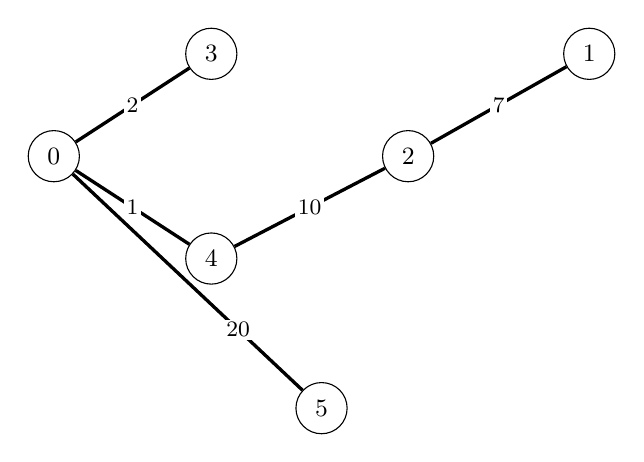
\begin{tikzpicture}[
    v/.style={circle, draw, minimum size=6.5mm, inner sep=0pt, font=\small},
    w/.style={fill=white, inner sep=1pt, font=\footnotesize}]
\node[v] (0) at (0,0) {0};
\node[v] (3) at (2,1.3) {3};
\node[v] (4) at (2,-1.3) {4};
\node[v] (2) at (4.5,0) {2};
\node[v] (1) at (6.8,1.3) {1};
\node[v] (5) at (3.4,-3.2) {5};
\draw[very thick] (0) -- node[w] {1} (4);
\draw[very thick] (0) -- node[w] {2} (3);
\draw[very thick] (4) -- node[w] {10} (2);
\draw[very thick] (2) -- node[w] {7} (1);
\draw[very thick] (0) -- node[w, pos=0.72] {20} (5);
\end{tikzpicture}
\end{center}
最低成本 $1 + 2 + 10 + 7 + 20 = 40$。

用 Kruskal 檢查：由輕到重 1 (0,4)、2 (0,3) 加入，3 (3,4) 成環丟掉，7 (1,2)、10 (2,4) 加入，
15 (2,3) 成環丟掉，20 (0,5) 加入，共五條，總和也是 40。 九條邊的權重都不同，最小擴張樹唯一
（資結書定理~24.4）。
\end{pastsoln}
